\section{Auswertung}

\subsection{Bragg-Bedingung}

Als erstes wird die Bragg-Bedingung überprüft. Dazu wird der Kristall auf einen Winkel von $\theta = 14^\circ$ eingestellt. Anschließend werden mit dem Geiger-Müller-Zählrohr für verschiedene Winkel jeweils 5s die eingehenden Impulse gemessen. Dies geschieht in einem Winkelbereich von $\theta = 26^\circ-\theta = 30^\circ$. Die aufgenommenen Messwerte sind in Tabelle \ref{tab:1}. Diese werden dann graphisch dargestellt und die Lage des Bragg-Peaks wurde ermittelt und markiert. 

Wie in Abbildung \ref{fig:Bragg} zu sehen ist liegt das gemessene Bragg-Peak bei $\theta = 28.2^\circ$. Mit dem Reflexionsgesetz ergibt sich der theoretische Sollwinkel von $\theta = 28^\circ$.

\begin{figure}
    \centering
    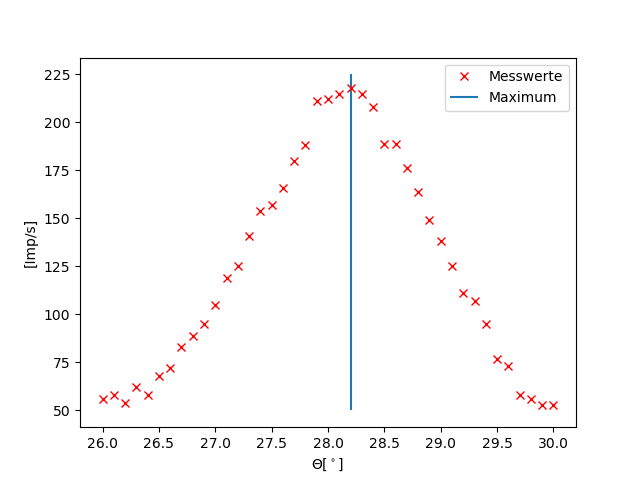
\includegraphics{bragg.png}
    \captionof{figure}{Graphische Darstellung der gemessenen Impulse N bei verschiedenen Winkeln $\theta$.}
    \label{fig:Bragg}
\end{figure}

\subsection{Emissionsspektrum der Kupfer-Röntgenröhre}

Die Messwerte für das Emissionsspektrum der Kupfer-Röntgenröhre sind in Tabelle \ref{tab:2}. Diese wurden anschließend graphisch dargestellt in Abbildung \ref{fig:copper}. Darin sind auch schon die K$_\text{\alpha}$- und die K$_\text{\beta}$-Linie, sowie deren Halbwertsbreiten eingetragen. 
Die Winkel der K-Linien betragen

\begin{align*}
    \theta_\text{\alpha} = \SI[separate-uncertainty=true]{22.5(0.2)}{\degree} \\
    \theta_\text{\beta} = \SI[separate-uncertainty=true]{20.2(0.2)}{\degree}.
\end{align*}

Aus diesen Winkeln können mithilfe der Bragg-schen Bedingung Wellenlängen berechnet werrden, die widerum mit $E=\frac{hc}{\lambda e}$ in Energien in Elektronenvolt umgerechnet werden können. Die entstehenden Energien sind

\begin{align*}
    E_\text{\alpha} = \SI[separate-uncertainty=true]{8.04(0.07)E3}{\electronvolt} \\
    E_\text{\beta} = \SI[separate-uncertainty=true]{8.91(0.08)E3}{\electronvolt}.
\end{align*}

Ebenso sind in dem Diagramm die beiden Halbwertsbreiten zu sehen. Die Halbwertsbreite des K$_\text{\alpha}$ Peaks wird durch die Winkel 

\begin{align*}
    \theta_\text{\alpha, links} = \SI[separate-uncertainty=true]{22.4(0.2)}{\degree} \\
    \theta_\text{\alpha, rechts} = \SI[separate-uncertainty=true]{22.9(0.2)}{\degree}
\end{align*}

begrenzt. Für das K$_\text{\beta}$-Peak sind die begrenzenden Winkel 

\begin{align*}
    \theta_\text{\beta, links} = \SI[separate-uncertainty=true]{20.2(0.2)}{\degree} \\
    \theta_\text{\beta, rechts} = \SI[separate-uncertainty=true]{20.6(0.2)}{\degree}
\end{align*}

Mit den Halbwertsbreiten können nun analog Energien bestimmt werden. Die dabei entstehenden Energien sind

\begin{align*}
    \Delta E_\text{FHWM,\alpha} = \SI[separate-uncertainty=true]{1.7(0.9)E2}{\electronvolt} \\
    \Delta E_\text{FHWM,\beta} = \SI[separate-uncertainty=true]{1.7(1.2)E2}{\electronvolt}.
\end{align*}

Daraus lässt sich nun das Auflösungsvermögen $A=\frac{E_\text{K}}{\Delta E_\text{FHWM}}$ berechnen zu 

\begin{align*}
    A_\text{K$_\alpha$} = 48 \pm 27 \\
    A_\text{K$_\beta$} = 50 \pm 40.
\end{align*}

Mit der Absorptionsenergie $E_\text{abs}$ \cite{Eabs} und den zuvor bestimmten Energien können nun die Absorptionskoeffizienten bestimmt werden. Die Absorptionskoeffizienten lauten 

\begin{align*}
    \sigma_1 = z-\sqrt{\frac{E_\text{abs}}{R_\infty}} = 3.30 \\
    \sigma_2 = z-2\cdot \sqrt{\frac{E_\text{abs}-E_\text{\alpha}}{R_\infty}} = 12.4\pm 0.6 \\
    \sigma_3 = z-3\cdot \sqrt{\frac{E_\text{abs}-E_\text{\beta}}{R_\infty}} = 22\pm 4 \\
\end{align*}

\begin{figure}
    \centering
    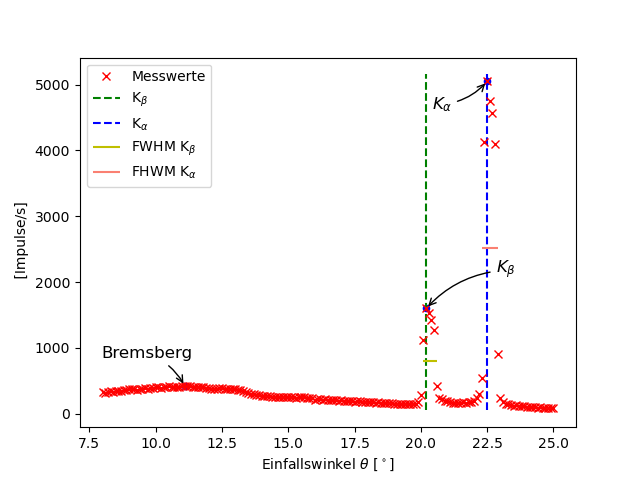
\includegraphics{copper.png}
    \captionof{figure}{Emissionsspektrum der Kupfer-Röntgenröhre.}
    \label{fig:copper}
\end{figure}

\subsection{Analyse der Absorptionsspektren}

Im folgenden wird für verschiedene Materialien die Absorptionsenergie bestimmt. Dafür wird zunächst die Intensität der Mitte der Kante $I_\text{K} = I_\text{K}^{min} + \frac{I_\text{K}^{max}-I_\text{K}^{min}}{2}$ bestimmt. Anschließend wird zwischen den beiden Punkten, die dieser Mitte am nächsten sind eine Gerade gezogen. Damit kann dann der Winkel bestimmt werden bei dem die gesuchte Intensität erreicht ist. Mit der Geradengleichung $I = a \cdot \theta + b$ ergibt sich der gesuchte Winkel zu $\theta_\text{K} = \frac{I_\text{K}-b}{a}$.

Dann wird dieser Winkel mit der zuvor beschriebenen Vorgehensweise in die Energie umgerechnet um dann abschließend die Abschirmkonstante 

\begin{equation*}
    \sigma_\text{K} = z-\sqrt{\frac{E_\text{K}}{R_\infty}-\frac{\alpha^2\cdot Z^4}{4}}
\end{equation*}

zu bestimmen.

\subsubsection{Brom}

Für das Absorptionsspektrum von Brom sind die Messdaten in Tabelle \ref{tab:3}. Der dazugehörige plot ist Abbildung \ref{fig:br}.

Das Maximum, das Minimum und die daraus resultierende Mitte der Kante ergeben sich hier zu 

\begin{align*}
    I_\text{min} = 9 \, Imp/s \\
    I_\text{max} = 27 \, Imp/s \\
    I_\text{K} = 18 \, Imp/s.
\end{align*}

Mit den Parametern der durch die beiden Punkte gelegten Gerade

\begin{align*}
    a = 40 \, Imp/s^\circ \\
    b = -511 Imp/s
\end{align*}

ergibt sich $\theta = 13.225  ^\circ$. Damit lassen sich nun die gesuchten Werte für die Absorptionsenergie und die Abschirmkonstante berechnen zu 

\begin{align*}
    E_\text{br} = \SI{13454.48}{\electronvolt}\\
    \sigma_\text{br} = 3.866.
\end{align*}

\begin{figure}
    \centering
    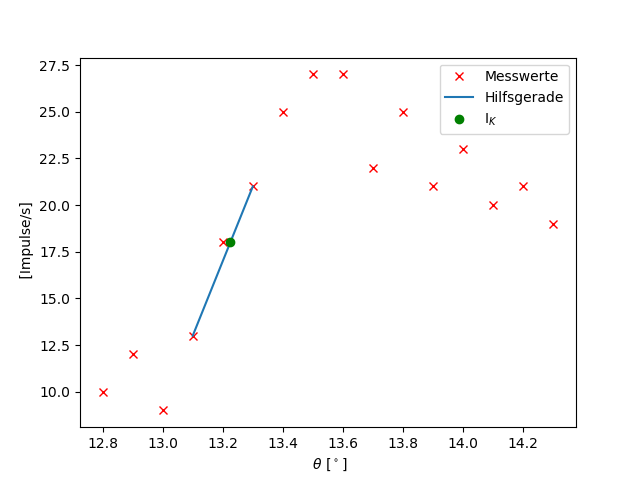
\includegraphics{br.png}
    \captionof{figure}{Absorptionsspektrum des Brom Absorbers.}
    \label{fig:br}
\end{figure}

\subsubsection{Gallium}

Die Messwerte der Messreihe mit dem Gallium- Absorber sind in Tabelle \ref{tab:4} und Abbildung \ref{fig:ga}. 

\begin{figure}
    \centering
    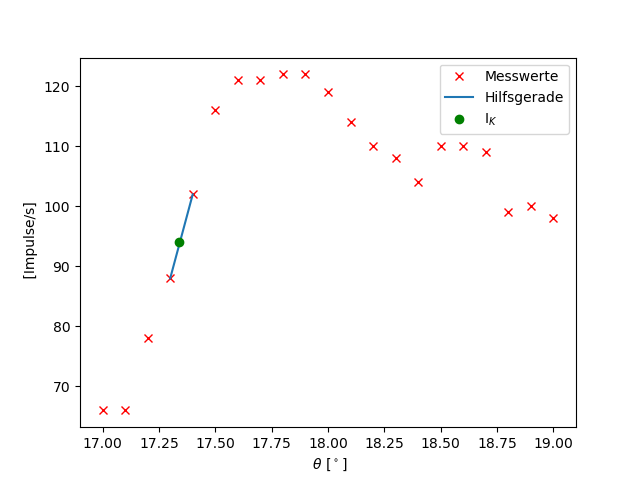
\includegraphics{ga.png}
    \captionof{figure}{Absorptionsspektrum des Gallium Absorbers.}
    \label{fig:ga}
\end{figure}

Diesmal sind die benötigten Intensitäten

\begin{align*}
    I_\text{min} = 66 \, Imp/s \\
    I_\text{max} = 122 \, Imp/s \\
    I_\text{K} = 94 \, Imp/s.
\end{align*}

Die bestimmten Parameter sind

\begin{align*}
    a = 140 \, Imp/s^\circ \\
    b = -2334 Imp/s.
\end{align*}

Daraus lassen sich nun $\theta = 17.34  ^\circ$, $E_\text{Ga} = 10325.97 \, eV$ und $\sigma_\text{Ga} = 3.669$

\subsubsection{Rubidium}

Das Diagramm für den Rubidium-Absorber ist in Abbildung \ref{fig:rb}. Die Messwerte dazu befinden sich in Tabelle \ref{tab:5}. Die Intensitäten haben bei diesem Absorber die Werte  

\begin{align*}
    I_\text{min} = 10 \, Imp/s \\
    I_\text{max} = 64 \, Imp/s \\
    I_\text{K} = 37 \, Imp/s.
\end{align*}

Mit den Parametern

\begin{align*}
    a = 70 \, Imp/s^\circ \\
    b = -787 Imp/s.
\end{align*}

lassen sich die gesuchten Werte 

\begin{align*}
    \theta = 11.77  ^\circ \\
    E_\text{rb} = \SI{15087.94}{\electronvolt}\\
    \sigma_\text{rb} = 4.069.
\end{align*}

bestimmen.

\begin{figure}
    \centering
    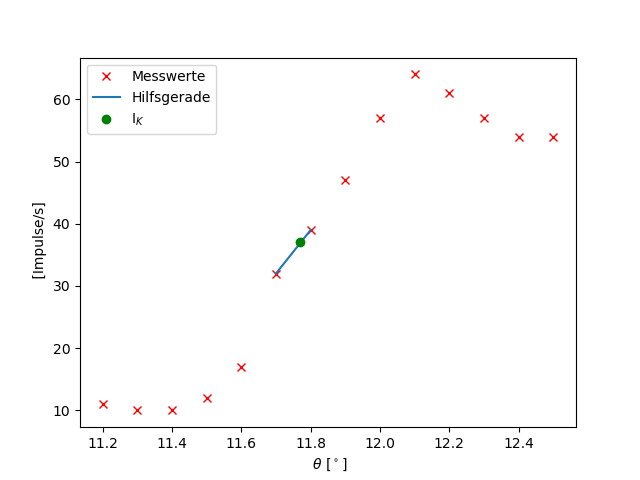
\includegraphics{rb.png}
    \captionof{figure}{Absorptionsspektrum des Rubidium Absorbers.}
    \label{fig:rb}
\end{figure}

\subsubsection{Strontium}

Die Messwerte der Messreihe mit dem Strontium- Absorber sind in Tabelle \ref{tab:6} und Abbildung \ref{fig:sr}. 

\begin{figure}
    \centering
    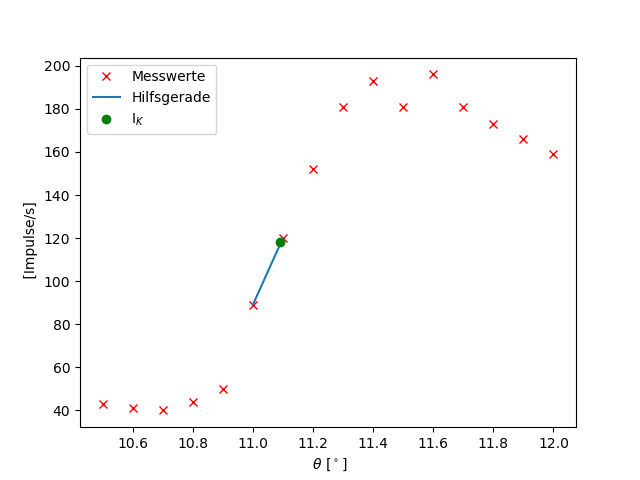
\includegraphics{sr.png}
    \captionof{figure}{Absorptionsspektrum des Gallium Absorbers.}
    \label{fig:sr}
\end{figure}

Diesmal sind die benötigten Intensitäten

\begin{align*}
    I_\text{min} = 40 \, Imp/s \\
    I_\text{max} = 196 \, Imp/s \\
    I_\text{K} = 118 \, Imp/s.
\end{align*}

Die bestimmten Parameter sind

\begin{align*}
    a = 310 \, Imp/s^\circ \\
    b = -3321 Imp/s.
\end{align*}

Daraus lassen sich nun $\theta = 11.09  ^\circ$, $E_\text{Ga} = 15997.27 \, eV$ und $\sigma_\text{Ga} = 4.11$

\subsubsection{Zink}

Das Diagramm für den Zink-Absorber ist in Abbildung \ref{fig:zn}. Die Messwerte dazu befinden sich in Tabelle \ref{tab:7}. Die Intensitäten haben bei diesem Absorber die Werte  

\begin{align*}
    I_\text{min} = 54 \, Imp/s \\
    I_\text{max} = 102 \, Imp/s \\
    I_\text{K} = 78 \, Imp/s.
\end{align*}

Mit den Parametern

\begin{align*}
    a = 190 \, Imp/s^\circ \\
    b = -3469 Imp/s.
\end{align*}

lassen sich die gesuchten Werte 

\begin{align*}
    \theta = 18.67  ^\circ \\
    E_\text{zn} = \SI{9616.20}{\electronvolt}\\
    \sigma_\text{zn} = 3.613
\end{align*}

berechnen.

\begin{figure}
    \centering
    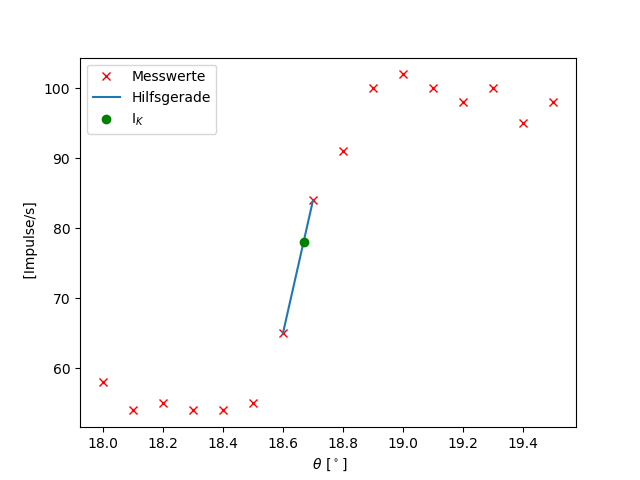
\includegraphics{zn.png}
    \captionof{figure}{Absorptionsspektrum des Zink Absorbers.}
    \label{fig:zn}
\end{figure}

\subsubsection{Zirkonium}

Für das Absorptionsspektrum von Zirkonium sind die Messdaten in Tabelle \ref{tab:8}. Der dazugehörige plot ist Abbildung \ref{fig:zr}.

Das Maximum, das Minimum und die daraus resultierende Mitte der Kante ergeben sich hier zu 

\begin{align*}
    I_\text{min} = 40 \, Imp/s \\
    I_\text{max} = 196 \, Imp/s \\
    I_\text{K} = 118 \, Imp/s.
\end{align*}

Mit den Parametern der durch die beiden Punkte gelegten Gerade

\begin{align*}
    a = 450 \, Imp/s^\circ \\
    b = -4275 Imp/s
\end{align*}

ergibt sich $\theta = 9.96  ^\circ$. Damit lassen sich nun die gesuchten Werte für die Absorptionsenergie und die Abschirmkonstante berechnen zu 

\begin{align*}
    E_\text{zr} = \SI{17798.26}{\electronvolt}\\
    \sigma_\text{zr} = 4.298.
\end{align*}

\begin{figure}
    \centering
    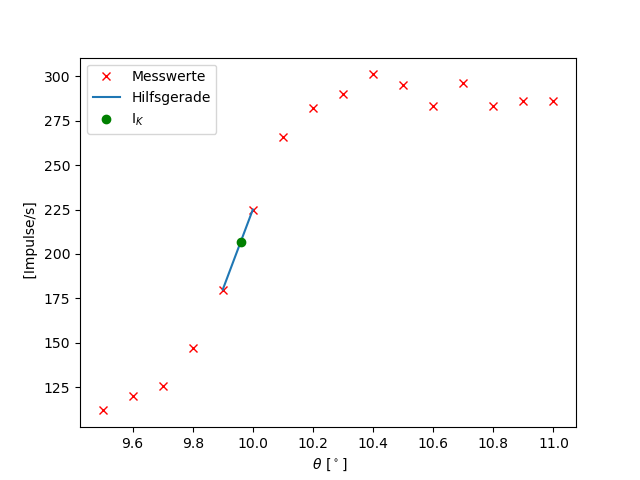
\includegraphics{zr.png}
    \captionof{figure}{Absorptionsspektrum des Zirkonium Absorbers.}
    \label{fig:zr}
\end{figure}

\subsection{Rydbergenergie}

Für die Bestimmung der Rydbergenergie wurde das Diagramm in Abblidung \ref{fig:ryd} erstellt. In der Abbildung wurde die Ordnungszahl gegen die Wurzel der Absorptionsenergie des jeweiligen Elements aufgetragen. Außerdem wurde eine lineare Ausgleichsrechnung durchgeführt. Die in der Abbildung zu sehende Ausgleichsgerade hat die Parameter 

\begin{align*}
    a = 0.283 \pm 0.001 \, \frac{1}{\sqrt{eV}} \\
    b = 2.277 \pm 0.121.
\end{align*}

Die Rydberenergie lässt sich mit dem Mosleyschen-Gesetz

\begin{equation*}
    R_\infty \cdot h = \frac{1}{a^2}
\end{equation*}

berechnen. Diese Rechnung liefert 

\begin{equation*}
    R_\infty = (12.5\pm 0.9)\, eV.
\end{equation*}

\begin{figure}
    \centering
    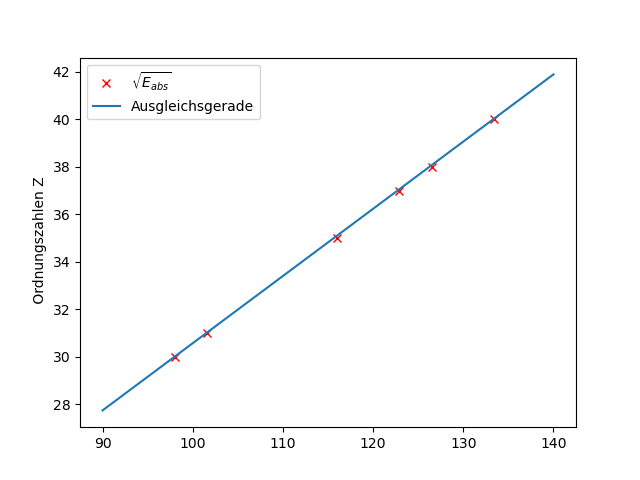
\includegraphics{ryd.png}
    \captionof{figure}{Plot zur Bestimmung der Rydberenergie.}
    \label{fig:ryd}
\end{figure}

\section{Diskussion}

\subsection{Bragg-Bedingung}

In diesem Experiment sollte die Bragg-Bedingung überprüft werden. Der gemessene Wert für den Winkel, bei dem das Bragg-Peak liegt ist $\theta = 28.2^\circ$. Der theoretische Sollwinkel liegt bei 28$^\circ$. Das ergibt eine prozentuale Abweichung von

\begin{equation*}
    \Delta \% = \frac{|28-28.2|}{28} = 0.7 \%.
\end{equation*}

Diese sehr geringe Abweichung lässt sich als erfolgreiche Überprüfung der Bragg-Bedingung interpretieren. Eine große Abweichung hätte zu Folge gehabt, dass es einen systematischen Fehler gibt der sich durch alle Messungen dieses Experiments durchzieht. 

\subsection{Emissionspektrum der Kupfer Röntgenröhre}

Die im Experiment bestimmten Werte für die Energien der K-Linien sind 

\begin{align*}
    E_\text{\alpha} = \SI[separate-uncertainty=true]{8.04(0.07)E3}{\electronvolt} \\
    E_\text{\beta} = \SI[separate-uncertainty=true]{8.91(0.08)E3}{\electronvolt}.
\end{align*}

Die Theoriewerte dazu sind:

\begin{align*}
    E_\text{\alpha} = \SI[separate-uncertainty=true]{8109}{\electronvolt} \\
    E_\text{\beta} = \SI[separate-uncertainty=true]{8.914}{\electronvolt}.
\end{align*}

Die prozentualen Abweichungen sind:

\begin{align*}
    \Delta E_\text{\alpha} = 0.85\% \\
    \Delta E_\text{\beta} = 0.04\%
\end{align*}

Die Abweichungen sind sehr gering. 

\subsection{Abschirmkonstanten}

In Tabelle \ref{tab:s} sind alle Abschirmkonstanten mit den dazugehörigen Theoriewerten und der prozentualen Abweichung von diesen angegeben. Die abweichung fallen auch hier insgesamt wieder sehr gering aus. Die vorhandenen Abweichungen könnten dadurch entstehen, dass kein kontinuirliches Spektrum an Winkeln gemessen werden kann. Durch eine Erhöhung der Auflösung könnten vorhandene Abweichungen weiter minimiert werden.

\begin{minipage}{\linewidth}
\begin{table}[H]
        \centering
    \captionof{table}{Abweichung der Abschirmkonstanten}
    \begin{tabular}{llll}
        \toprule
        Material & $\sigma_\text{Exp}$ & $\sigma_\text{Theo}$& Abweichung [\%] \\
        \midrule
        Brom        & 3.866 & 3.84 & 0.7 \\
        Gallium     & 3.670 & 3.62 & 1.38 \\
        Rubidium    & 4.069 & 3.95 & 3.01 \\
        Strontium   & 4.110 & 3.99 & 3.00 \\
        Zink        & 3.613 & 3.56 & 1.49 \\
        Zirkonium   & 4.298 & 4.39 & 2.10 \\
        \bottomrule   
    \end{tabular}
    
    \label{tab:s}
\end{table}
\end{minipage}

\subsection{Rydbergenergie}

Die experimentell bestimmte Rydberenergie hat einen Wert von $R_\infty = (12.5\pm 0.9)\, eV$. Diese weicht um 8.09\% von dem Theoriewert von $R_\infty = 13.6\, eV$ ab.
Die Abweichung fällt hier etwas höher aus, als die Abweichung bei den vorherigen Werten. Dies ist nicht verwunderlich, da diese Rydbergenergie aus diesen Werten bestimmt wurde und die Fehler der anderen Werte sich auf diesen neuen Wert übertragen und vervielfachen.
    


\section{Messwerte}

\begin{minipage}{\linewidth}
    \begin{table}[H]
        \centering
    \captionof{table}{Messwerte zur Überprüfung der Bragg-Bedingung}
    \begin{tabular}{lll}
        \toprule
        $\theta [^\circ]$ & N [Imp/s] \\
        \midrule
        26.0  &	56.0  \\
        26.1  &	58.0  \\
        26.2  &	54.0  \\
        26.3  &	62.0  \\
        26.4  &	58.0  \\
        26.5  &	68.0  \\
        26.6  &	72.0  \\
        26.7  &	83.0  \\
        26.8  &	89.0  \\
        26.9  &	95.0  \\
        27.0  &	105.0 \\
        27.1  &	119.0 \\
        27.2  &	125.0 \\
        27.3  &	141.0 \\
        27.4  &	154.0 \\
        27.5  &	157.0 \\
        27.6  &	166.0 \\
        27.7  &	180.0 \\
        27.8  &	188.0 \\
        27.9  &	211.0 \\
        28.0  &	212.0 \\
        28.1  &	215.0 \\
        28.2  &	218.0 \\
        28.3  &	215.0 \\
        28.4  &	208.0 \\
        28.5  &	189.0 \\
        28.6  &	189.0 \\
        28.7  &	176.0 \\
        28.8  &	164.0 \\
        28.9  &	149.0 \\
        29.0  &	138.0 \\
        29.1  &	125.0 \\
        29.2  &	111.0 \\
        29.3  &	107.0 \\
        29.4  &	95.0  \\
        29.5  &	77.0  \\
        29.6  &	73.0  \\
        29.7  &	58.0  \\
        29.8  &	56.0  \\
        29.9  &	53.0  \\
        30.0  &	53.0  \\
        \bottomrule   
    \end{tabular}
    
    \label{tab:1}
\end{table}
\end{minipage}


\begin{minipage}{\linewidth}
    \begin{table}[H]
        \centering
    \captionof{table}{Messwerte für das Emissionsspektrum der Kupfer-Röntgenröhre}
    \begin{tabular}{lll}
        \toprule
        $\theta [^\circ]$ & N [Imp/s] \\
        \midrule
        8.0		& 323.0 \\
        8.1		& 316.0 \\
        8.2		& 326.0 \\
        8.3		& 340.0 \\
        8.4		& 335.0 \\
        8.5		& 343.0 \\
        8.6		& 350.0 \\
        8.7		& 350.0 \\
        8.8		& 366.0 \\
        8.9		& 357.0 \\
        9.0		& 371.0 \\
        9.1		& 371.0 \\
        9.2		& 372.0 \\
        9.3		& 364.0 \\
        9.4		& 381.0 \\
        9.5		& 379.0 \\
        9.6		& 393.0 \\
        9.7		& 375.0 \\
        9.8		& 391.0 \\
        9.9		& 395.0 \\
        10.0	& 402.0 \\
        10.1	& 405.0 \\
        10.2	& 390.0 \\
        10.3	& 398.0 \\
        10.4	& 400.0 \\
        10.5	& 418.0 \\
        10.6	& 401.0 \\
        10.7	& 410.0 \\
        10.8	& 408.0 \\
        10.9	& 409.0 \\
        11.0	& 414.0 \\
        11.1	& 420.0 \\
        11.2	& 417.0 \\
        11.3	& 417.0 \\
        11.4	& 409.0 \\
        11.5	& 406.0 \\
        11.6	& 404.0 \\
        11.7	& 405.0 \\
        11.8	& 400.0 \\
        11.9	& 383.0 \\
        12.0	& 389.0 \\
        12.1	& 382.0 \\
        12.2	& 372.0 \\
        12.3	& 376.0 \\
        12.4	& 385.0 \\
        12.5	& 384.0 \\
        12.6	& 382.0 \\
        12.7	& 373.0 \\
        12.8	& 376.0 \\
        12.9	& 373.0 \\
        13.0	& 375.0 \\
        13.1	& 366.0 \\
        13.2	& 354.0 \\
        13.3	& 341.0 \\
        13.4	& 326.0 \\
        13.5	& 318.0 \\
        13.6	& 305.0 \\
        13.7	& 296.0 \\
        13.8	& 286.0 \\
        13.9	& 285.0 \\
        14.0	& 274.0 \\
        14.1	& 264.0 \\
        14.2	& 266.0 \\
        14.3	& 270.0 \\
        14.4	& 255.0 \\
        14.5	& 255.0 \\
        14.6	& 260.0 \\
        14.7	& 251.0 \\
        14.8	& 250.0 \\
        14.9	& 248.0 \\
        15.0	& 253.0 \\
        15.1	& 257.0 \\
        15.2	& 248.0 \\
        15.3	& 242.0 \\
        15.4	& 249.0 \\
        15.5	& 246.0 \\
        15.6	& 252.0 \\
        15.7	& 236.0 \\
        15.8	& 234.0 \\
        15.9	& 231.0 \\
        16.0	& 215.0 \\
        16.1	& 217.0 \\
        16.2	& 227.0 \\
        16.3	& 214.0 \\
        16.4	& 217.0 \\
        16.5	& 210.0 \\
        16.6	& 211.0 \\
        16.7	& 206.0 \\
        16.8	& 205.0 \\
        16.9	& 198.0 \\
        17.0	& 203.0 \\
        17.1	& 199.0 \\
        17.2	& 198.0 \\
        17.3	& 191.0 \\
        17.4	& 192.0 \\
        17.5	& 184.0 \\
        17.6	& 191.0 \\
        17.7	& 188.0 \\
        17.8	& 181.0 \\
        17.9	& 185.0 \\
        18.0	& 184.0 \\
        18.1	& 179.0 \\
        18.2	& 180.0 \\
        18.3	& 166.0 \\
        18.4	& 173.0 \\
        18.5	& 167.0 \\
        18.6	& 169.0 \\
        18.7	& 160.0 \\
        18.8	& 159.0 \\
        18.9	& 157.0 \\
        19.0	& 149.0 \\
        19.1	& 153.0 \\
        19.2	& 150.0 \\
        19.3	& 147.0 \\
        19.4	& 150.0 \\
        19.5	& 148.0 \\
        19.6	& 149.0 \\
        19.7	& 143.0 \\
        19.8	& 153.0 \\
        19.9	& 182.0 \\
        20.0	& 291.0 \\
        20.1	& 1127.0 \\
        20.2	& 1599.0 \\
        20.3	& 1533.0 \\
        20.4	& 1430.0 \\
        20.5	& 1267.0 \\
        20.6	& 425.0 \\
        20.7	& 241.0 \\
        20.8	& 225.0 \\
        20.9	& 192.0 \\
        21.0	& 188.0 \\
        21.1	& 172.0 \\
        21.2	& 168.0 \\
        21.3	& 169.0 \\
        21.4	& 166.0 \\
        21.5	& 170.0 \\
        21.6	& 174.0 \\
        21.7	& 164.0 \\
        21.8	& 180.0 \\
        21.9	& 179.0 \\
        22.0	& 191.0 \\
        22.1	& 232.0 \\
        22.2	& 300.0 \\
        22.3	& 536.0 \\
        22.4	& 4128.0 \\
        22.5	& 5050.0 \\ 
        22.6	& 4750.0 \\
        22.7	& 4571.0 \\
        22.8	& 4097.0 \\
        22.9	& 901.0 \\
        23.0	& 244.0 \\
        23.1	& 179.0 \\
        23.2	& 151.0 \\
        23.3	& 145.0 \\
        23.4	& 130.0 \\
        23.5	& 121.0 \\
        23.6	& 126.0 \\
        23.7	& 117.0 \\
        23.8	& 112.0 \\
        23.9	& 110.0 \\
        24.0	& 105.0 \\
        24.1	& 106.0 \\
        24.2	& 107.0 \\
        24.3	& 95.0 \\
        24.4	& 94.0 \\
        24.5	& 100.0 \\
        24.6	& 91.0 \\
        24.7	& 85.0 \\
        24.8	& 88.0 \\
        24.9	& 83.0 \\
        25.0	& 85.0 \\
        \bottomrule   
    \end{tabular}
    
    \label{tab:2}
\end{table}
\end{minipage}

\begin{minipage}{\linewidth}
    \begin{table}[H]
        \centering
    \captionof{table}{Messwerte für das Absorptionsspektrum des Brom Absorbers}
    \begin{tabular}{lll}
        \toprule
        $\theta [^\circ]$ & N [Imp/s] \\
        \midrule
        12.8 & 	10.0 \\
        12.9 &	12.0 \\
        13.0 &	9.0  \\
        13.1 &	13.0 \\
        13.2 &	18.0 \\
        13.3 &	21.0 \\
        13.4 &	25.0 \\
        13.5 &	27.0 \\
        13.6 &	27.0 \\
        13.7 &	22.0 \\
        13.8 &	25.0 \\
        13.9 &	21.0 \\
        14.0 &	23.0 \\
        14.1 &	20.0 \\
        14.2 &	21.0 \\
        14.3 &	19.0 \\
        \bottomrule   
    \end{tabular}
    
    \label{tab:3}
\end{table}
\end{minipage}

\begin{minipage}{\linewidth}
    \begin{table}[H]
        \centering
    \captionof{table}{Messwerte für das Absorptionsspektrum des Gallium Absorbers}
    \begin{tabular}{lll}
        \toprule
        $\theta [^\circ]$ & N [Imp/s] \\
        \midrule
        17.0  &	66.0  \\
        17.1  &	66.0  \\
        17.2  &	78.0  \\
        17.3  &	88.0  \\
        17.4  &	102.0 \\
        17.5  &	116.0 \\
        17.6  &	121.0 \\
        17.7  &	121.0 \\
        17.8  &	122.0 \\
        17.9  &	122.0 \\
        18.0  &	119.0 \\
        18.1  &	114.0 \\
        18.2  &	110.0 \\
        18.3  &	108.0 \\
        18.4  &	104.0 \\
        18.5  &	110.0 \\
        18.6  &	110.0 \\
        18.7  &	109.0 \\
        18.8  &	99.0  \\
        18.9  &	100.0 \\
        19.0  &	98.0  \\
        \bottomrule   
    \end{tabular}
    
    \label{tab:4}
\end{table}
\end{minipage}

\begin{minipage}{\linewidth}
    \begin{table}[H]
        \centering
    \captionof{table}{Messwerte für das Absorptionsspektrum des Rubidium Absorbers}
    \begin{tabular}{lll}
        \toprule
        $\theta [^\circ]$ & N [Imp/s] \\
        \midrule
        11.2  &	11.0 \\
        11.3  &	10.0 \\
        11.4  &	10.0 \\
        11.5  &	12.0 \\
        11.6  &	17.0 \\
        11.7  &	32.0 \\
        11.8  &	39.0 \\
        11.9  &	47.0 \\
        12.0  &	57.0 \\
        12.1  &	64.0 \\
        12.2  &	61.0 \\
        12.3  &	57.0 \\
        12.4  &	54.0 \\
        12.5  &	54.0 \\
        \bottomrule   
    \end{tabular}
    
    \label{tab:5}
\end{table}
\end{minipage}

\begin{minipage}{\linewidth}
    \begin{table}[H]
        \centering
    \captionof{table}{Messwerte für das Absorptionsspektrum des Strontium Absorbers}
    \begin{tabular}{lll}
        \toprule
        $\theta [^\circ]$ & N [Imp/s] \\
        \midrule
        10.5  &	43.0  \\
        10.6  &	41.0  \\
        10.7  &	40.0  \\
        10.8  &	44.0  \\
        10.9  &	50.0  \\
        11.0  &	89.0  \\
        11.1  &	120.0 \\
        11.2  &	152.0 \\
        11.3  &	181.0 \\
        11.4  &	193.0 \\
        11.5  &	181.0 \\
        11.6  &	196.0 \\
        11.7  &	181.0 \\
        11.8  &	173.0 \\
        11.9  &	166.0 \\
        12.0  &	159.0 \\
        \bottomrule   
    \end{tabular}
    
    \label{tab:6}
\end{table}
\end{minipage}

\begin{minipage}{\linewidth}
    \begin{table}[H]
        \centering
    \captionof{table}{Messwerte für das Absorptionsspektrum des Zink Absorbers}
    \begin{tabular}{lll}
        \toprule
        $\theta [^\circ]$ & N [Imp/s] \\
        \midrule
        18.0  & 58.0 \\
        18.1  & 54.0 \\
        18.2  & 55.0 \\
        18.3  & 54.0 \\
        18.4  & 54.0 \\
        18.5  & 55.0 \\
        18.6  & 65.0 \\
        18.7  & 84.0 \\
        18.8  & 91.0 \\
        18.9  & 100.0 \\
        19.0  & 102.0 \\
        19.1  & 100.0 \\
        19.2  & 98.0 \\
        19.3  & 100.0 \\
        19.4  & 95.0 \\ 
        19.5  & 98.0 \\
        \bottomrule   
    \end{tabular}
    
    \label{tab:7}
\end{table}
\end{minipage}